\clearpage
\section{Checklisten}
\label{bkm:Ref2018102501}

Das Modul 'Checklisten' unterstützt Sie im Abarbeiten von Prüfpunkten bei Begehungen oder Abnahmen. Im Voraus wird eine Checkliste erstellt, welche x-beliebige 'Items' (Prüfpunkte) enthält. Die fertige Checkliste kann im Sitzungswesen bei Traktanden oder beim Anforderungs- und Mängelmanagement bei Vorbehalten verknüpft werden.

\begin{itemize}
\item
\textbf{Sitzungswesen:} Mittels einer Sitzung kann eine Begehung abgebildet werden. Die Beteiligten werden als Teilnehmer erfasst, die Traktanden entsprechen den verschiedenen Themenbereichen einer Begehung. Eine Checkliste mit den enthaltenen Prüfpunkten wird bei einem Traktandum verknüpft.
\item
\textbf{Vorbehalte beim Anforderungs- und Mängelmanagement:} Eine oder mehrere Checklisten können bei einem Vorbehalt verknüpft werden.
\end{itemize}

Für die Checklisten, resp. die Prüfpunkte wird ein Statussystem konfiguriert, welches sich an den vorgegebenen Prozessen orientiert. Beispielsweise kann ein einfaches Statussystem aus 'OK', 'offen' und 'Nicht OK' bestehen.

\vspace{\baselineskip}

Die Besonderheit der Checklisten ist, dass diese Mobile-tauglich sind. Checklisten können mit Smartphones oder Tablets abgearbeitet werden. Bei einer Begehung wird pro Prüfpunkt ein Status gesetzt, ergänzt mit einem Kommentar und wo nötig kann ein Foto oder Dokument hinzugefügt werden.\\
Da alles online bearbeitet wird, stehen die erfassten Daten umgehend zur weiteren Verarbeitung oder dem Erstellen eines Berichts zur Verfügung.

\vspace{\baselineskip}

% \begin{wrapfigure}[3]{l}{6.5cm}   % [x] Wie manche Zeile soll sich um die Grafik "brechen"
%   \vspace{-35pt}      % Grundwert war 20; mit 30 schön oben beim Text ausgerichtet
%   \begin{center}
%     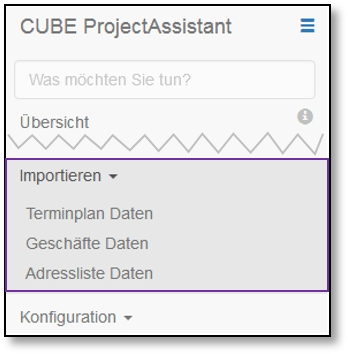
\includegraphics[width=1\linewidth]{../chapters/12_Importieren/pictures/12_Menu_Importieren.jpg}
%   \end{center}
%   \vspace{-20pt}
%   \caption{Daten importieren}
%   \vspace{-10pt}
% \end{wrapfigure}

Wählen Sie im Menü links unter 'Sitzungswesen' oder 'Anforderungs- und Mängelmanagement' den Punkt 'Checklisten' aus. Folgende Übersicht erscheint:

\begin{figure}[H]
\center{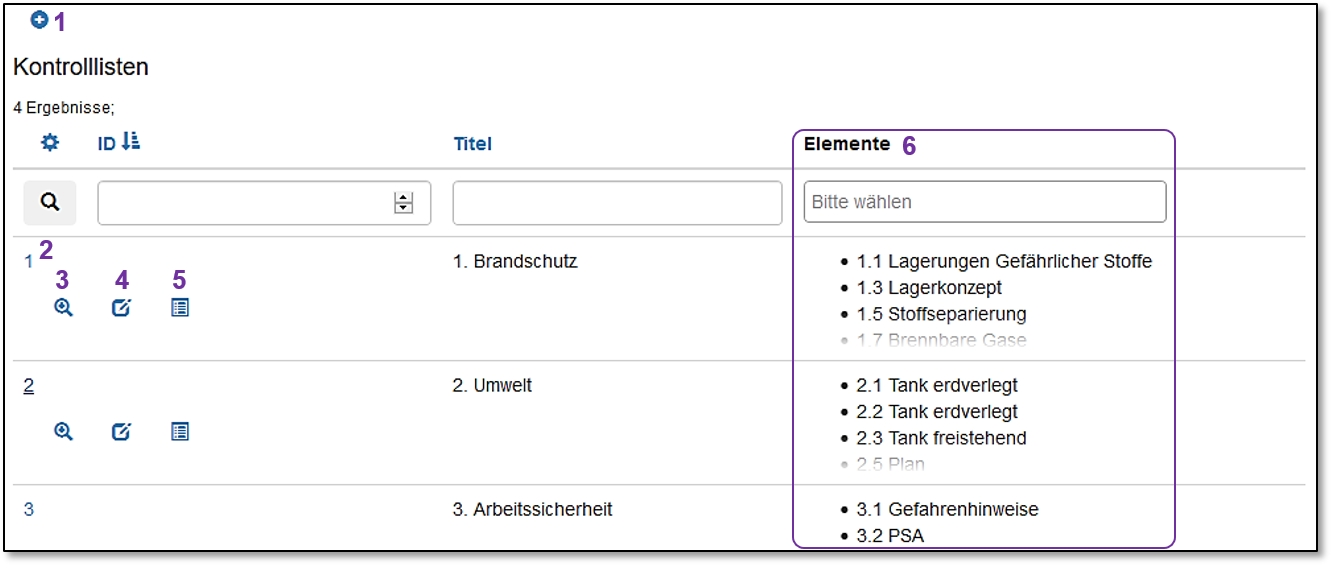
\includegraphics[width=1\linewidth]{../chapters/06_Checklisten/pictures/chl_ChecklisteUebersicht.jpg}}
\caption{Checklisten in der Übersicht}
% \label{fig:speciation}
\end{figure}

Mit den Filterfeldern können Sie nach ID, Titel und Elemente suchen (Begriffe eingeben und die Lupe 
\includegraphics[height=12pt]{/Icons/Lupe_kl.jpg} klicken) und mit Klick auf den blauen Titelnamen die angezeigten Datensätze von A-Z oder Z-A sortieren.\\
Wenn Sie eine neue Checkliste erstellen wollen, klicken Sie auf das Plussymbol 
\includegraphics[height=12pt]{/Icons/Plussymbol.jpg} \col{(1)}. Mehr dazu im nächsten Kapitel.\\
Mit Klick auf die 'ID' \col{(2)} einer Checklsite werden die Optionen geöffnet (erneuter Klick schliesst die Optionen wieder). Klicken Sie auf die kleine Lupe 
\includegraphics[height=12pt]{/Icons/Lupe.jpg} \col{(3)}, um die Checkliste im Betrachtungsmodus anzuschauen oder auf das Bearbeitensymbol 
\includegraphics[height=12pt]{/Icons/Bearbeiten.jpg} \col{(4)}, um die Checkliste zu ändern.\\
Von der Checklistenübersicht aus wird die Validierung einer Checkliste mit Klick auf das Listensymbol 
\includegraphics[height=12pt]{/Icons/Listensymbol.jpg} \col{(5)} gestartet.\\
Unter 'Elemente' sehen Sie Items / Prüfpunkte einer Checkliste und können mit dem Dropdownmenü nach einem gewünschten Item suchen (Auswahl des entsprechenden Items oder freie Texteingabe).\\
Mit Klick auf die ausgegraute Stelle wird die komplette Auflistung angezeigt.

\subsection{Checklisten erstellen}

Klicken Sie in der Checklisten-Übersicht auf das Plussymbol 
\includegraphics[height=12pt]{/Icons/Plussymbol.jpg}. Nun  können Sie eine neue Checkliste erstellen:

\begin{figure}[H]
\center{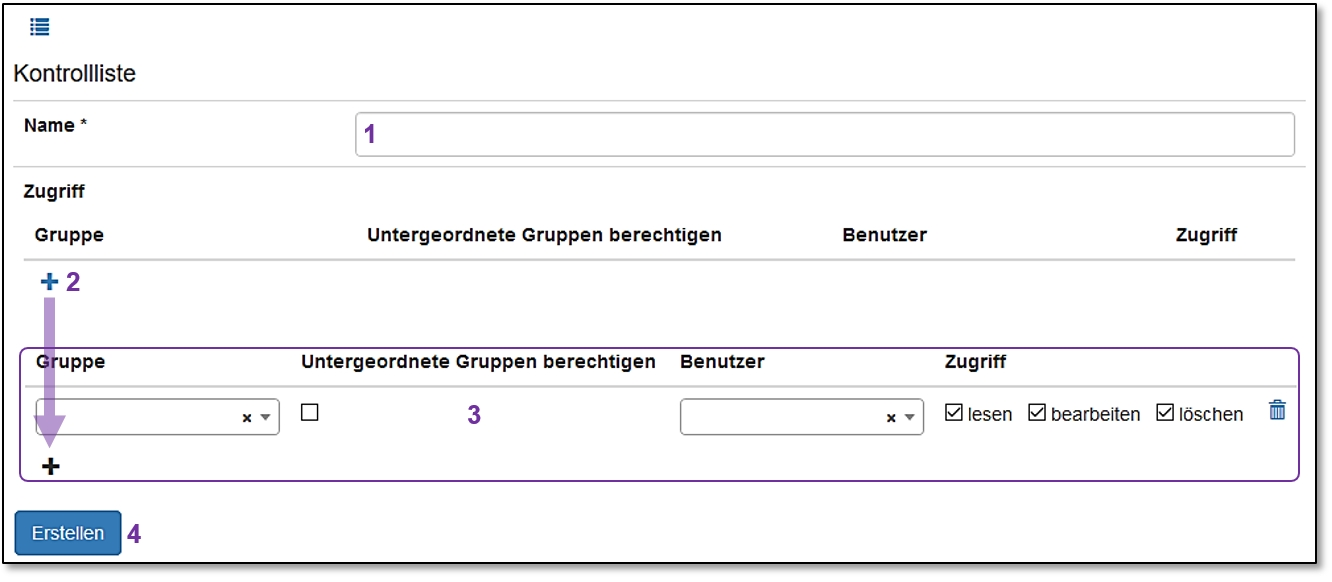
\includegraphics[width=1\linewidth]{../chapters/06_Checklisten/pictures/chl_NeueCheckliste.jpg}}
\caption{Neue Checkliste erstellen}
% \label{fig:speciation}
\end{figure}

Geben Sie der Checklsite einen passenden Titel \col{(1)} und erstellen Sie die benötigten Zugriffsrechte.

\vspace{\baselineskip}

\textbf{Hinweis:} Damit Sie die Berechtigungen einstellen können, müssen Sie auf das Plussymbol 
\includegraphics[height=12pt]{/Icons/Pluszeichen.jpg} \col{(2)} klicken. Nun werden die Eingabefelder ersichtlich.

\vspace{\baselineskip}

Sie können eine ganze Gruppe berechtigen oder einzelne Benutzer. Mindestens ein Benutzer benötigt sämtliche Rechte (lesen, bearbeiten, löschen). Überzählige Berechtigungsvergaben lassen sich mit dem Mülltonnensymbol 
\includegraphics[height=12pt]{/Icons/Muelltonne.jpg} wieder löschen.

\subsection{Items/Prüfpunkte erstellen}

Nachdem Sie den Button 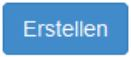
\includegraphics[height=12pt]{/Icons/B_Erstellen.jpg} geklickt haben, können nun die einzelnen Items / Prüfpunkte hinzugefügt werden:

\begin{figure}[H]
\center{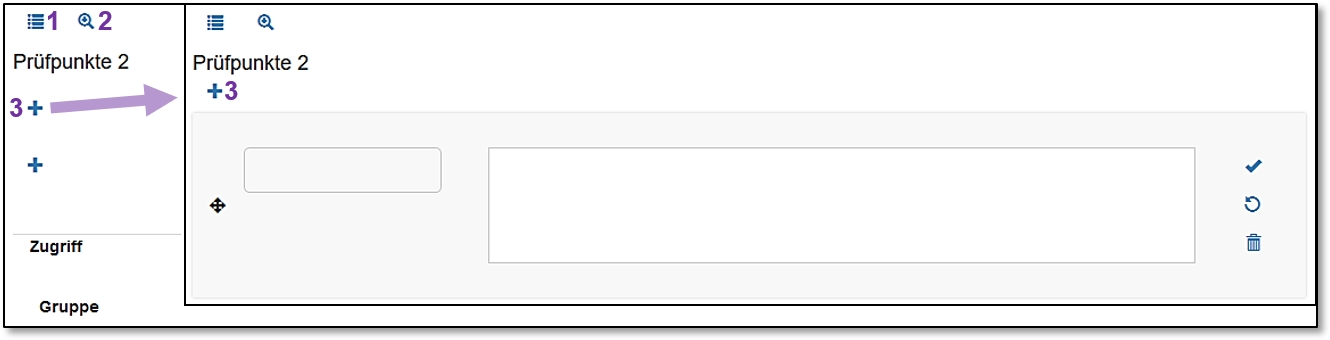
\includegraphics[width=1\linewidth]{../chapters/06_Checklisten/pictures/chl_NeueItems.jpg}}
\caption{Neue Items / Prüfpunkte hinzufügen}
% \label{fig:speciation}
\end{figure}

(Mit Klick auf das Listensymbol 
\includegraphics[height=12pt]{/Icons/Listensymbol_zurueck.jpg} \col{(1)} gelangen Sie wieder auf die Übersicht der Checklisten. Klicken Sie auf die Lupe 
\includegraphics[height=12pt]{/Icons/Lupe.jpg} \col{(2)}, um in den Ansichtsmodus zu wechseln.)

\vspace{\baselineskip}

Zuerst klicken Sie auf der leeren Maske auf das Plussymbol 
\includegraphics[height=12pt]{/Icons/Pluszeichen.jpg} \col{(3)}, um ein neues Item / ein neuer Prüfpunkt zu erzeugen:

\pagebreak

\begin{figure}[H]
\center{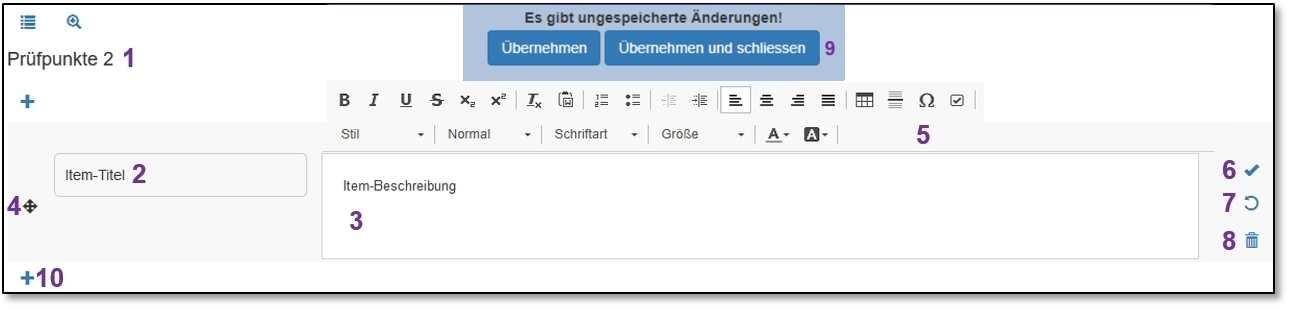
\includegraphics[width=1\linewidth]{../chapters/06_Checklisten/pictures/chl_NeueItemsFunktionen.jpg}}
\caption{Neue Items - Funktionsübersicht}
% \label{fig:speciation}
\end{figure}

\textbf{Die Funktionen im Überblick}

\vspace{\baselineskip}

\begin{tabular}{| p{3cm} | p{12cm} |} %{cl}
	% {|t | l p{8cm} | l}
\hline
\col{(1)} Titel der Checkliste & Sie können den Titel hier direkt anpassen, indem Sie mit der Maus zwischen die Buchstaben klicken und die Änderungen vornehmen. Speichern Sie die Änderungen mit {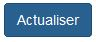
\includegraphics[height=12pt]{/Icons/B_Uebernehmen.jpg}} ab \col{(9)} \\
\hline
\col{(2)} Item-Titel & Geben Sie einem Item / einem Prüfpunkt einen passenden Titel und speichern Sie diesen mit {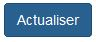
\includegraphics[height=12pt]{/Icons/B_Uebernehmen.jpg}} \col{(9)} oder dem Gutzeichen {
\includegraphics[height=12pt]{/Icons/Gutzeichen.jpg}} \col{(6)} ab. \\
\hline
\col{(3)} Item-Beschreibung & Nun können Sie das Item / der Prüfpunkt näher beschreiben und den Text formatieren \col{(5)}. Speichern Sie diesen mit {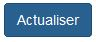
\includegraphics[height=12pt]{/Icons/B_Uebernehmen.jpg}} \col{(9)} oder dem Gutzeichen 
\includegraphics[height=12pt]{/Icons/Gutzeichen.jpg} \col{(6)} ab. \\
\hline
\col{(4)} Item verschieben & Die Item können in der Reihenfolge geändert werden. Packen Sie das 
\includegraphics[height=12pt]{/Icons/verschieben.jpg}-Symbol mit linker Maustaste und verschieben Sie das Item nach oben oder unten.\\
\hline
\col{(5)} Formatierung und Sonderfunktionen & Die Item Beschreibung können Sie formatieren oder Sonderfunktionen wie Checkboxen, Links, Tabellen und weitere hinzufügen. \\
\hline
\col{(6)} Einzelnes Item speichern & Ein neues Item oder Änderungen eines bestehendem Item werden mit Klick auf das Gutzeichen 
\includegraphics[height=12pt]{/Icons/Gutzeichen.jpg} \col{(6)} gespeichert. \\
\hline
\col{(7)} Änderungen verwerfen & Haben Sie Änderungen vorgenommen, welche Sie nicht behalten möchten, können Sie mit dem 
\includegraphics[height=12pt]{/Icons/Refresh.jpg}-Symbol \col{(7)} diese Änderungen verwerfen. Der letzte gespeicherte Zustand wird wiederherstellt. \\
\hline
\col{(8)} Items löschen & Wenn Sie ein Item nicht mehr benötigen, können Sie es mittels dem Mülltonnen-Symbol (
\includegraphics[height=12pt]{/Icons/Refresh.jpg}) \col{(8)} löschen. \\
\hline
\col{(9)} Änderungen übernehmen & Alternativ zum Speichern mittels dem Gutzeichen (
\includegraphics[height=12pt]{/Icons/Gutzeichen.jpg}) können Sie sämtliche Änderungen auf der Webseite mit dem 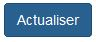
\includegraphics[height=12pt]{/Icons/B_Uebernehmen.jpg}-Button speichern. \\
\hline
\col{(10)} Neues Item erstellen & Klicken Sie auf das Plussymbol (
\includegraphics[height=12pt]{/Icons/Pluszeichen.jpg}), um ein neues / weiteres Item zu erstellen. Das neue Item wird immer zuunterst erstellt. Sie haben zu Beginn der Items und unterhalb des letzten Items ein 
\includegraphics[height=12pt]{/Icons/Pluszeichen.jpg}-Symbol, um weitere Items zu erstellen. \\
\hline
\end{tabular}

\subsection{Checklisten verknüpfen}

Checklisten lassen sich im Sitzungswesen bei den Traktanden oder im Anforderungs - und Mängelmanagement bei den Vorbehalten verknüpfen.

\vspace{\baselineskip}

\subsubsection{Checklisten verknüpfen beim Sitzungswesen}

\begin{figure}[H]
\center{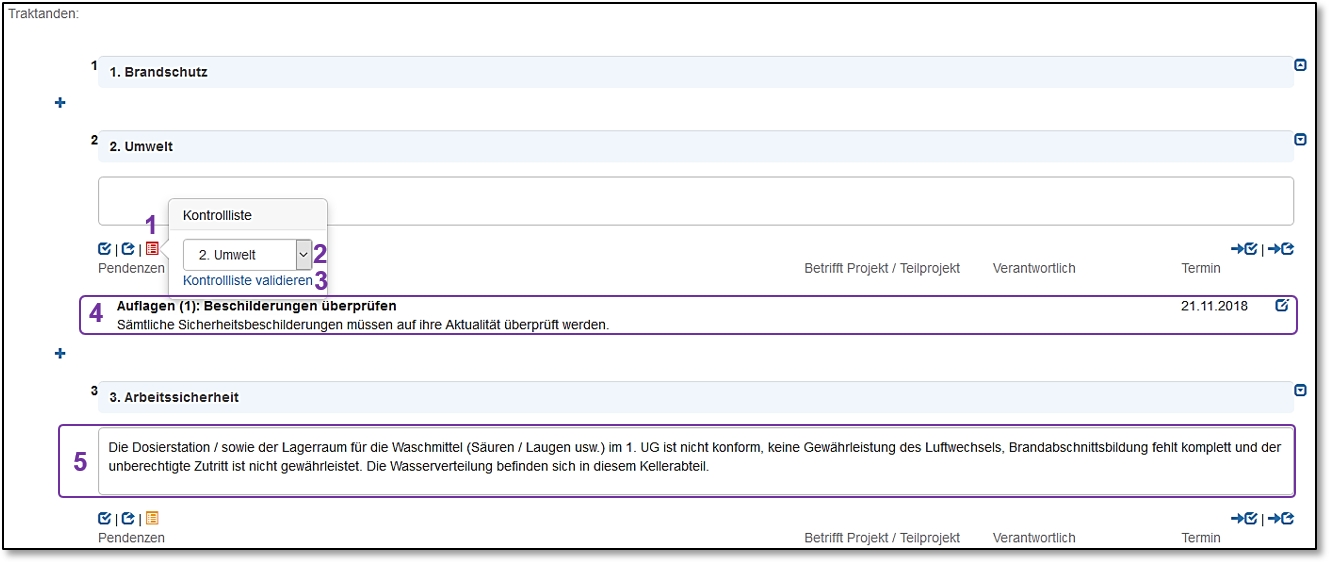
\includegraphics[width=1\linewidth]{../chapters/06_Checklisten/pictures/chl_verkTraktanden.jpg}}
\caption{Checklisten beim Sitzungswesen in den Traktanden verknüpfen}
% \label{fig:speciation}
\end{figure}

Im Sitzungswesen können Sie eine Begehung als Sitzung organisieren, die Anwesenden als Teilnehmer einladen und das Begehungsprogramm mittels den Traktanden abbilden. Zu jedem Traktandum lässt sich eine Checkliste verknüpfen \col{(1)}. Mittels dem Dropdownmenü \col{(2)} wird die Checkliste ausgewählt und mit Klick auf den Textlink 'Kontrollliste validieren' wird die Checkliste im Validierungsmodus geöffnet (siehe Kapitel \ref{bkm:Ref2018102901})

\vspace{\baselineskip}

Offene Punkte bei einer Checkliste, resp. einem Prüfpunkt können mittels Pendenzen aufgenommen und mit Termin und Verantwortlichkeit ergänzt werden \col{(4)}. Eine Zusammenfassung der Begehung kann mit der Protokollierfunktion gleich ins Begehungsprotokoll aufgenommen werden.

\subsubsection{Checklisten verknüpfen bei den Vorbehalten}

\begin{figure}[H]
\center{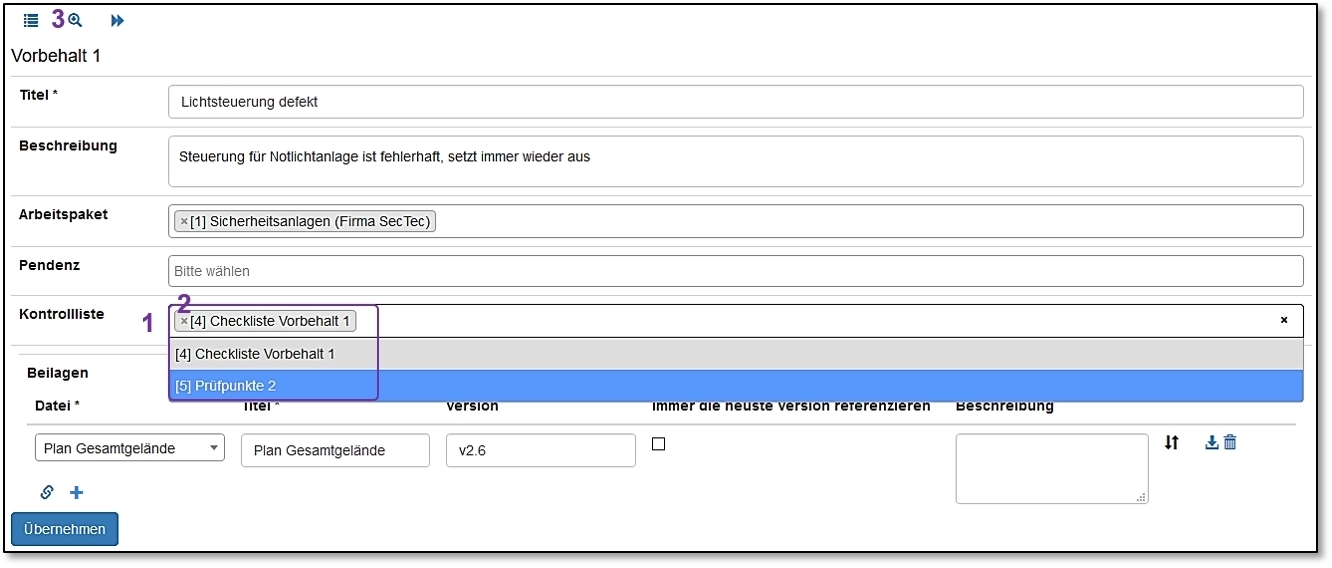
\includegraphics[width=1\linewidth]{../chapters/06_Checklisten/pictures/chl_verkVorbehalte.jpg}}
\caption{Checklisten bei den Vorbehalten verknüpfen}
% \label{fig:speciation}
\end{figure}

Öffnen Sie im Anforderungs- und Mängelmanagement-Modul den gewünschte Vorbehalt. Unter 'Kontrollliste' \col{(1)} können die zur Verfügung stehenden Checklisten verknüpft werden. Dabei ist eine Mehrfachauswahl möglich. Mit dem 'x' \col{(2)} lassen sich überzählige Checklisten-Verknüpfungen wieder löschen.\\
Wechseln Sie in den Betrachtungsmodus \col{(3)} kann die Validierungsansicht einer Checkliste aufgerufen werden:

\begin{figure}[H]
\center{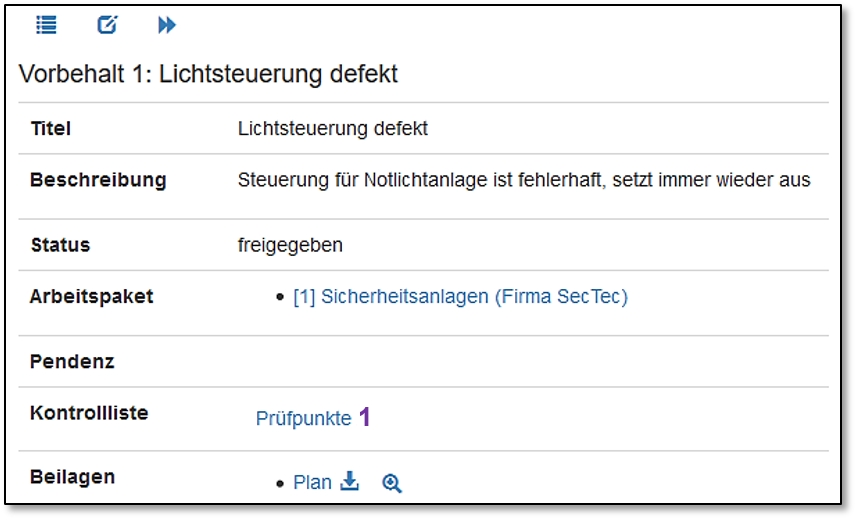
\includegraphics[width=.6\linewidth]{../chapters/06_Checklisten/pictures/chl_VorbView.jpg}}
\caption{Checklisten bei den Vorbehalten verknüpfen}
% \label{fig:speciation}
\end{figure}

Klicken Sie auf den Textlink der entsprechenden Checkliste \col{(1)} Die Checkliste wird im Validierungsmodus geöffnet. Mehr in Kapitel \ref{bkm:Ref2018102901}.

\pagebreak

\subsection{Checklisten validieren}
\label{bkm:Ref2018102901}

Öffnen Sie die Validierung einer Checkliste:

\begin{wrapfigure}[19]{l}{9cm}   % [x] Wie manche Zeile soll sich um die Grafik "brechen"
  \vspace{-20pt}      % Grundwert war 20; mit 30 schön oben beim Text ausgerichtet
  \begin{center}
    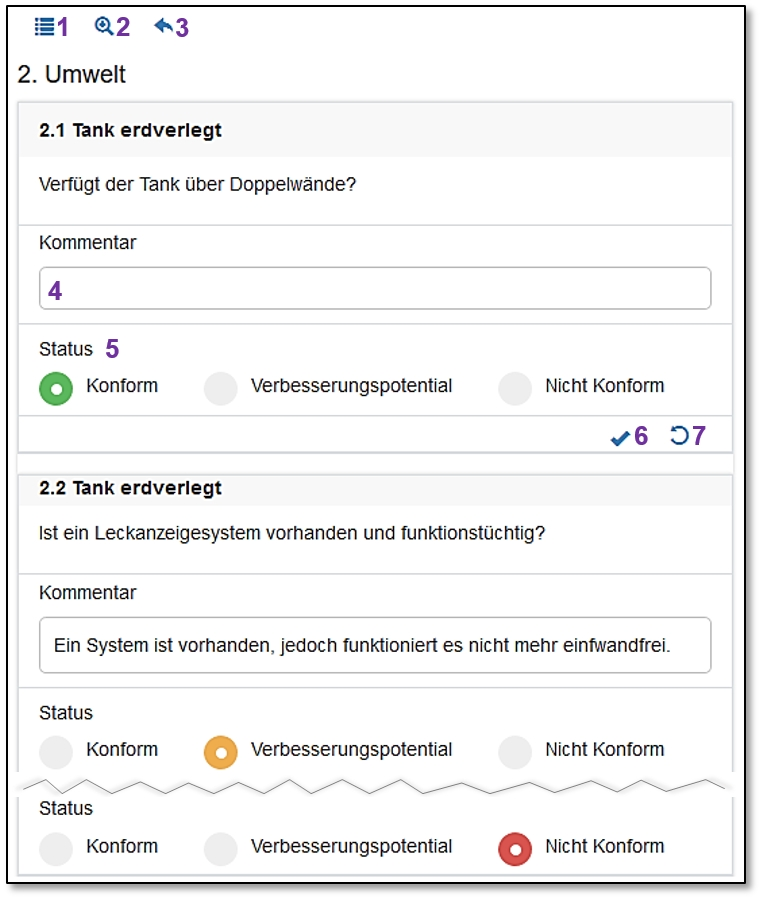
\includegraphics[width=1\linewidth]{../chapters/06_Checklisten/pictures/ckl_Validierung.jpg}
  \end{center}
  \vspace{-20pt}
  \caption{Validierung einer Checkliste}
  \vspace{-10pt}
\end{wrapfigure}

\textbf{Hinweis:} Das Statussystem einer Checkliste ist konfigurierbar und variiert in der Anzahl der Status und auch der Farbgebung.

\vspace{\baselineskip}

Mit Klick auf das Listensymbol 
\includegraphics[height=12pt]{/Icons/Listensymbol_zurueck.jpg}-Symbol \col{(1)} gelangen Sie in die Übersicht der Checklisten. Mit Klick auf die Lupe 
\includegraphics[height=12pt]{/Icons/Lupe.jpg}-Symbol \col{(2)} wird in den Betrachtungsmodus der geöffneten Checkliste gewechselt. \\
Wenn Sie auf das Pfeilsymbol klicken 
\includegraphics[height=12pt]{/Icons/Pfeil_l.jpg}-Symbol \col{(3)} gelangen Sie an die Stelle in CUBE PA, von welcher Sie die Validierung aufgerufen haben. Wurde die Checkliste im Sitzungswesen bei den Traktanden aufgerufen, wird mit Klick auf 
\includegraphics[height=12pt]{/Icons/Pfeil_l.jpg}-Symbol \col{(3)} wieder das Sitzungswesen aufgerufen.

\vspace{\baselineskip}

Bei Bedarf können Sie bei dem Prüfpunkt einen Kommentar hinterlegen \col{(4)}. Wählen Sie mit der Maus und einem Linksklick in den entsprechenden Kreis den gewünschten Status aus. Die Farbdefinition kann beliebig angepasst werden. Nehmen Sie dazu Kontakt mit dem CUBE PA Support auf.

\vspace{\baselineskip}

Soll ein Eintrag gespeichert werden, klicken Sie auf das Gutzeichen 
\includegraphics[height=12pt]{/Icons/Gutzeichen.jpg}-Symbol \col{(6)}. Sie können die getätigten Eingaben auch rückgängig machen mit Klick auf das Refresh-Icon 
\includegraphics[height=12pt]{/Icons/Refresh.jpg}-Symbol \col{(7)}. Die Änderungen gehen verloren.

\vspace{\baselineskip}

\textbf{Hinweis:} Wenn Sie mehrere Prüfpunkte bearbeiten und beispielsweise Kommentare eintragen, können Sie alle Änderungen pauschal mit der Schaltfläche oben im Bildschirm speichern:

\begin{figure}[H]
\center{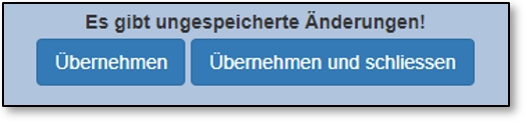
\includegraphics[width=.3\linewidth]{../chapters/06_Checklisten/pictures/ckl_Uebernehmen.jpg}}
% \caption{Checklisten bei den Vorbehalten verknüpfen}
% \label{fig:speciation}
\end{figure}
